To nie jest przyjemny dowód i jest absolutnie koszmarny do sformalizowania. Mimo wszystko spróbuję. W sumie to nawet nie jest dowód, to jest bardziej algorytm postępowania.

Zacznijmy na początku od zdefiniowania problemu.
Mamy graf \(G\) oraz zbiór wierzchołków, które z jakiegoś powodu nazywamy
\textit{terminalami}.
Bardzo chcielibyśmy znaleźć najmniejszy (krawędziowo) podgraf, który łączy wszystkie terminale.
Oczywiście widzimy, że musi być to drzewo (stąd nazwa), gdyż w przeciwnym razie moglibyśmy pozbyć się jakiejś krawędzi bez naruszania spójności.

\begin{figure}[H]
	\centering
	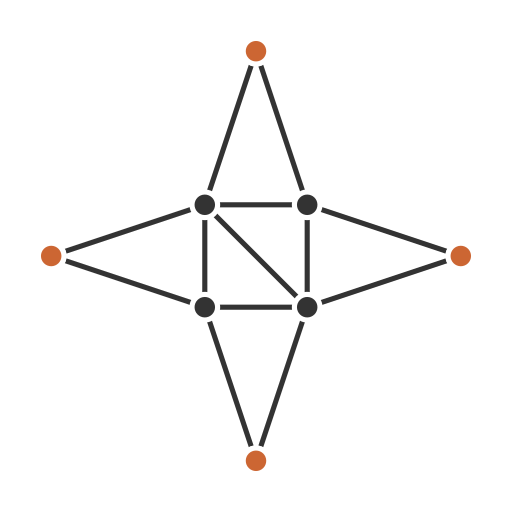
\includegraphics[scale=0.4]{images/steiner/steiner_problem_example.png}
	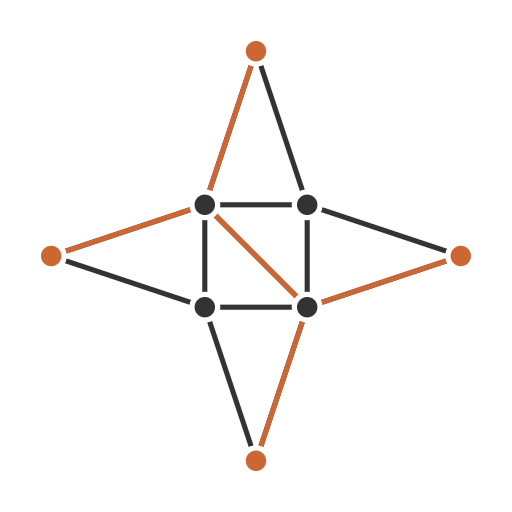
\includegraphics[scale=0.4]{images/steiner/steiner_problem_example_tree.png}
	\caption{Przykładowy graf z terminalami oraz minimalne drzewo je łączące}
\end{figure}


\textbf{Spacerem rozgałęziającym się} będziemy nazywać ukorzenione oraz uporządkowane (tzn. dzieci każdego wierzchołka są ponumerowane) drzewo, które ,,przerzucimy'' w dosyć dziwny sposób na graf w którym szukamy drzewa Steinera. Generalnie wierzchołki drzewa mapujemy dowolnie na wierzchołki grafu, z tym że jeśli 2 wierzchołki w drzewie są połączone krawędzią, to po przemapowaniu również muszą być połączone krawędzią. Co ważne, \textbf{wiele wierzchołków drzewa może zostać przemapowane na ten sam wierzchołek naszego grafu}. Intuicyjnie odpowiada to wielu równoległym spacerom z tego samego punktu.

Formalniej można o tym myśleć jak o krotce
\begin{equation*}
	(T, \pi, \varphi)
\end{equation*}
gdzie \(T\) jest jakimś drzewem, \(\pi\) permutacją dzięki której mamy porządek dzieci, a \(\varphi\) funkcją mapującą wierzchołki tego drzewa na nasz graf, zgodnie z warunkiem który został tu opisany.

Bardzo chcielibyśmy umieć liczyć sobie, ile jest spacerów rozgałęziających się o danej długości, ,,zaczynających'' się w danym wierzchołku. Okazuje się, że możemy to liczyć z pomocą programowania dynamicznego. Przed \(dp[v][i]\) będziemy oznaczać liczbę spacerów rozgałęziających się ,,wychodzących'' z wierzchołka \(v\) mających \(i\) krawędzi. Mamy, że:
\begin{equation*}
	dp[v][0] = 1
\end{equation*}
co jest dosyć oczywiste, bo skoro jest 0 krawędzi to ten spacer rozgałęziający się ma po prostu jeden wierzchołek i taki jest jeden.
Dosyć prosto też zaobserwować, że
\begin{equation*}
	dp[v][1] = deg(v)
\end{equation*}
Bo drzewo które będziemy chcieli zmapować na nasz graf będzie mieć 1 krawędź; tym samym jesteśmy w stanie przemapować jeden wierzchołek zawsze na wierzchołek \(v\), a drugi na któregoś z jego sąsiadów. Mało odkrywcza obserwacja i w sumie to bezużyteczna, bo wprost będzie wynikać ze wzoru który zostanie zaraz podany.

\begin{theorem}[Straszny wzór]
	\begin{equation}
		dp[u][i] = \sum_{v \in N(u)} \sum_{a+b=i-1} dp[u][a] \cdot dp[v][b]
	\end{equation}
\end{theorem}

\begin{proof}
	Tu trzeba by chyba było zacząć rysować, żeby to sensownie dowieść, ale generalnie chodzi o to że jak mamy drzewo i mapujemy je na nasz graf, to dziecko naszego korzenia (najbardziej na ,,lewo'' jak rozpiszemy graficznie) w swoim poddrzewie ma jakieś \(a\) krawędzi, a cała reszta drzewa ma jakieś \(b\) krawędzi. Jak się to narysuje to widać, że \(a + b = n-1\), bo krawędź łącząca korzeń z lewym dzieckiem łączyła 2 rozpatrywane przez nas poddrzewa, które teraz rozpatrujemy osobno. Teraz liczba spacerów rozgałęziających się to po prostu suma po wszystkich możliwych wierzchołkach na które mapujemy tamto dziecko i możliwych wartościach \(a, b\) i iloczynach spacerów \(dp[u][a]\) i \(dp[v][b]\) czyli liczbach spacerów rozgałęziających się długości \(a\) z tego dziecka i długości \(b\) z całej reszty. Wartości te już mamy policzone, więc to jest poprawnie zdefiniowane. Obliczenie wszystkich możliwych tych wartości działa jakoś wielomianowo.

	\begin{figure}[H]
		\centering
		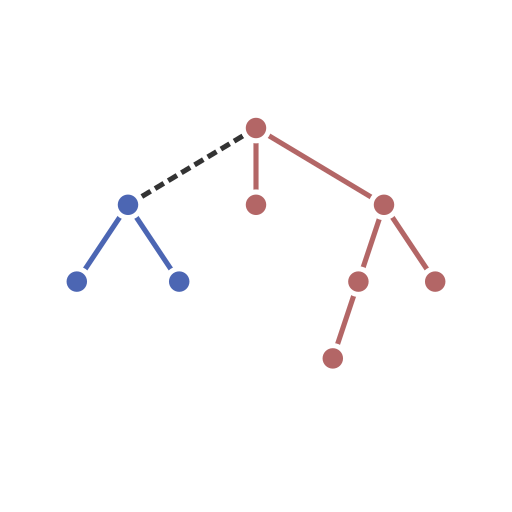
\includegraphics[scale=0.4]{images/steiner/steiner_dp_example_1.png}
		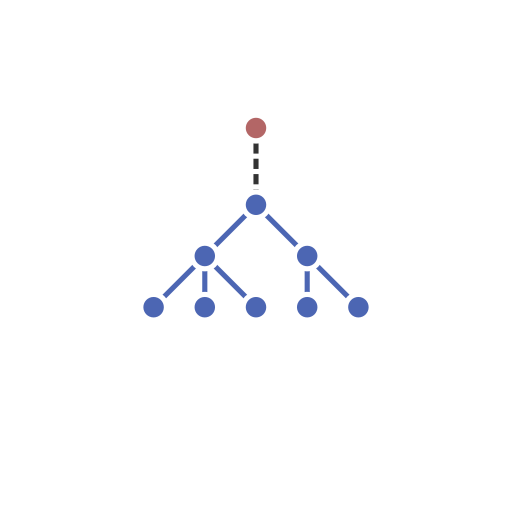
\includegraphics[scale=0.4]{images/steiner/steiner_dp_example_2.png}
		\caption{Przykłady podziału spaceru na dwie części. \\ Po lewej \(a = 2, b = 5\), po prawej \(a = 7, b = 0\)}
	\end{figure}
\end{proof}

Z tego wzoru istotnie wynika wcześniejsza obserwacja, bo \begin{equation*}
	dp[u][1] = \sum_{v \in N(u)}\sum_{a+b = 0} dp[u][a] \cdot dp[v][b] = \sum_{v \in N(u)} dp[u][0] \cdot dp[v][0] = \sum_{v \in N(u)} 1 \cdot 1 = deg(u)
\end{equation*}

Teraz zaczniemy używać motywów bardzo podobnych do tych występujących w problemie zliczania liczby cyklów Hamiltona w grafie. Mianowicie, przez \(U\) oznaczę sobie zbiór wszystkich spacerów rozgałęziających się, wychodzących z jakiegoś terminala \(t\) oraz mapujących dokładnie \(l\) krawędzi (innymi słowy, drzewo musi mieć \(l\) krawędzi, a funkcja przesyłająca musi przesyłać jego korzeń na \(t\)). Poza tym, zakładam że w grafie mam jakieś terminale \(t_1, t_2, \dots, t_k\) (gdy terminal jest tylko jeden, problem znalezienia drzewa Steinera jest dosyć trywialny). Przez \(A_i\) oznaczam zbiór wszystkich spacerów rozgałęziających się z \(U\), które mapują jakiś wierzchołek drzewa na terminal \(t_i\).

Zauważmy, że \(\bigcap_{i \in [k]} A_i \) da nam zbiór wszystkich spacerów rozgałęziających się, które można ,,przerobić'' do postaci drzewa łączącego wszystkie terminale, a więc jeśli jest niepusty to znaczy to, że istnieje drzewo łączące wszystkie terminale mające \(l\) krawędzi (lub mniej, ale to nam w tym problemie nie przeszkadza; chcemy wiedzieć czy istnieje drzewo łączące wszystkie terminale, mające maksymalnie l krawędzi).

Ponadto, żeby żyło się prościej, wprowadzam oznaczenie \(S_i = U - A_i\), Innymi słowy, \(S_i\) to zbiór wszystkich spacerów rozgałęziających się z \(U\), które nie mapują niczego na \(t_i\). Wykonuję teraz przekształcenia podobne do tych, które robiliśmy przy cyklach Hamiltona:
\begin{equation*}
	|\bigcap_{i \in [k]} A_i| = |U| - |\bigcup_{i \in [k]} U \setminus A_i| = |U| - |\bigcup_{i \in [k]} S_i|
\end{equation*}
\begin{equation*}
	|U| - |\bigcup_{i \in [k]} S_i| = |U| - \sum_{\emptyset \not = X \subset [k]} (-1)^{|X| - 1} \cdot |\bigcap_{i \in X} S_i|
\end{equation*}
Zasadniczo teraz mamy już skończony algorytm obliczania, bo:
\begin{enumerate}
	\item \(|U|\) jesteśmy w stanie obliczyć w czasie wielomianowym, bo to po prostu \(dp[t][l]\)
	\item \(|\bigcap_{i \in X} S_i|\) dla danego \(X\) również obliczamy w czasie wielomianowym, bo to jest \(dp[t][l]\) ale policzone dla grafu indukowanego bez wierzchołków, po których iterujemy się idąc przez \(X\). Innymi słowy, zbiór \(S_{i_1} \cap S_{i_2} \cap \dots \cap S_{i_j}\) jest to zbiór wszystkich spacerów rozgałęziających się w grafie \(G [V \setminus \{t_{i_1}, t_{i_2}, \dots, t_{i_j}\}] \).
\end{enumerate}
